\documentclass[tikz, border=2pt]{standalone}
\usepackage{amsmath,amssymb}
\usepackage{xcolor}
\usetikzlibrary{shapes.geometric, arrows.meta, positioning, calc, fit, backgrounds}

\definecolor{clientborder}{RGB}{30, 64, 175}
\definecolor{clientbg}{RGB}{241, 245, 249}
\definecolor{cardbg}{RGB}{255, 255, 255}
\definecolor{cloudborder}{RGB}{51, 65, 85}
\definecolor{cloudbg}{RGB}{248, 250, 252}
\definecolor{netborder}{RGB}{217, 119, 6}
\definecolor{netbg}{RGB}{255, 251, 235}
\definecolor{secgreen}{RGB}{4, 120, 87}
\definecolor{tagblue}{RGB}{224, 231, 255}
\definecolor{tagtext}{RGB}{30, 58, 138}
\definecolor{warnred}{RGB}{185, 28, 28}
\definecolor{warnbg}{RGB}{254, 242, 242}

\begin{document}

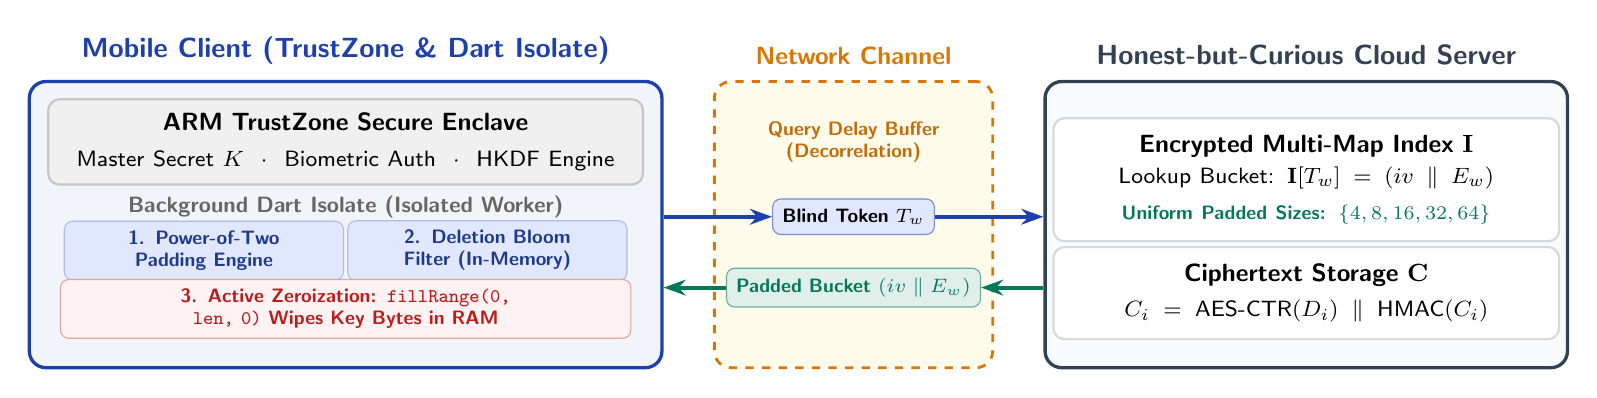
\begin{tikzpicture}[
    font=\small\sffamily,
    subcard/.style={draw=gray!30, fill=cardbg, rounded corners=4pt, line width=0.8pt, align=center, inner sep=6pt},
    tzstyle/.style={draw=gray!45, fill=gray!12, rounded corners=4pt, line width=0.8pt, align=center, inner sep=5pt},
    pill/.style={draw=clientborder!35, fill=tagblue, text=tagtext, rounded corners=3pt, font=\scriptsize\bfseries\sffamily, align=center, inner sep=3.5pt},
    warnpill/.style={draw=warnred!40, fill=warnbg, text=warnred, rounded corners=3pt, font=\scriptsize\bfseries\sffamily, align=center, inner sep=3.5pt},
    arrowblue/.style={-{Stealth[length=2.8mm, width=2.0mm]}, line width=1.4pt, draw=clientborder},
    arrowgreen/.style={-{Stealth[length=2.8mm, width=2.0mm]}, line width=1.4pt, draw=secgreen}
]

% ================= CLIENT COLUMN (Center x = 0) =================
\node[tzstyle, text width=7.2cm] (tz) at (0, 1.2) {
    \textbf{ARM TrustZone Secure Enclave}\\[2pt]
    \footnotesize Master Secret $K$ $\;\cdot\;$ Biometric Auth $\;\cdot\;$ HKDF Engine
};

\node[font=\footnotesize\bfseries\sffamily, text=gray!80!black] (iso_title) at (0, 0.38) {Background Dart Isolate (Isolated Worker)};

\node[pill, text width=3.3cm] (pad) at (-1.8, -0.18) {
    1. Power-of-Two\\Padding Engine
};

\node[pill, text width=3.3cm] (bloom) at (1.8, -0.18) {
    2. Deletion Bloom\\Filter (In-Memory)
};

\node[warnpill, text width=7.0cm] (zero) at (0, -0.92) {
    3. Active Zeroization: \texttt{fillRange(0, len, 0)} Wipes Key Bytes in RAM
};

% Isolate container
\begin{scope}[on background layer]
    \node[subcard, fit=(iso_title) (pad) (bloom) (zero), inner ysep=6pt, inner xsep=6pt] (iso_box) {};
\end{scope}

% Client Outer Container
\begin{scope}[on background layer]
    \node[draw=clientborder, fill=clientbg, rounded corners=6pt, line width=1.2pt, fit={( -3.9, -1.55) (3.9, 1.85)}] (client_box) {};
\end{scope}
\node[above=2pt of client_box.north, font=\normalsize\bfseries\sffamily, text=clientborder] {Mobile Client (TrustZone \& Dart Isolate)};

% ================= CLOUD SERVER (Center x = 12.2) =================
\node[subcard, text width=6.0cm] (idx_box) at (12.2, 0.72) {
    \textbf{Encrypted Multi-Map Index $\mathbf{I}$}\\[2pt]
    \footnotesize Lookup Bucket: $\mathbf{I}[T_w] = (iv \parallel E_w)$\\[2pt]
    \scriptsize\bfseries\sffamily\textcolor{secgreen}{Uniform Padded Sizes: $\{4, 8, 16, 32, 64\}$}
};

\node[subcard, text width=6.0cm] (store_box) at (12.2, -0.72) {
    \textbf{Ciphertext Storage $\mathbf{C}$}\\[2pt]
    \footnotesize $C_i = \text{AES-CTR}(D_i) \parallel \text{HMAC}(C_i)$
};

\begin{scope}[on background layer]
    \node[draw=cloudborder, fill=cloudbg, rounded corners=6pt, line width=1.2pt, fit={(9.0, -1.55) (15.4, 1.85)}] (cloud_box) {};
\end{scope}
\node[above=2pt of cloud_box.north, font=\normalsize\bfseries\sffamily, text=cloudborder] {Honest-but-Curious Cloud Server};

% ================= NETWORK CHANNEL (Center x = 6.45) =================
\begin{scope}[on background layer]
    \node[draw=netborder, fill=netbg, dashed, rounded corners=6pt, line width=1.0pt, fit={(4.8, -1.55) (8.1, 1.85)}] (net_box) {};
\end{scope}
\node[above=2pt of net_box.north, font=\small\bfseries\sffamily, text=netborder] {Network Channel};

\node[font=\scriptsize\bfseries\sffamily, text=netborder!90!black, align=center] at (6.45, 1.2) {Query Delay Buffer\\(Decorrelation)};

% Tokens inside Network Channel
\node[draw=clientborder!60, fill=tagblue, rounded corners=3pt, font=\scriptsize\bfseries\sffamily, inner sep=3.5pt] (tok_box) at (6.45, 0.25) {Blind Token $T_w$};

\node[draw=secgreen!60, fill=secgreen!12, text=secgreen, rounded corners=3pt, font=\scriptsize\bfseries\sffamily, inner sep=3.5pt] (pad_box) at (6.45, -0.65) {Padded Bucket $(iv \parallel E_w)$};

% ================= FLOW ARROWS =================
% Search Query Flow (Client -> Token -> Cloud)
\draw[arrowblue] (client_box.east |- tok_box) -- (tok_box.west);
\draw[arrowblue] (tok_box.east) -- (cloud_box.west |- tok_box);

% Search Response Flow (Cloud -> Bucket -> Client)
\draw[arrowgreen] (cloud_box.west |- pad_box) -- (pad_box.east);
\draw[arrowgreen] (pad_box.west) -- (client_box.east |- pad_box);

\end{tikzpicture}

\end{document}
